\documentclass[12pt]{article}

\usepackage{ulem}
\usepackage{float}
\usepackage{graphicx}
\usepackage{fancyhdr}
\usepackage{setspace}
\usepackage[hidelinks]{hyperref}
\usepackage[spanish]{babel}
\usepackage{mlmodern}
\usepackage{longtable}
\usepackage{tabularx}
\usepackage{multicol}
\usepackage[T1]{fontenc}
\usepackage[left=2cm, right=2cm, top=4cm, bottom=2.5cm, headheight=2cm, headsep=1cm]{geometry}
\renewcommand{\normalsize}{\fontsize{13}{15}\selectfont}

\pagestyle{fancy}
\fancyhead[C]
{
    \makebox[\textwidth]{
        \hspace{-0.2\textwidth}
        \begin{minipage}[c][2.5cm]{0.2\textwidth}
            
\includegraphics[width=2.5cm]{logo}
        \end{minipage}
        \hspace{0.01\textwidth}
        \begin{minipage}[c][2.5cm]{0.6\textwidth}
            \centering
            \textbf{\LARGE Colegio Bautista Libertad}\\[0.2cm]
            \textbf{\Large Capacitación docente 2025}\\
            Contacto: soporte@cbl-edu.com
        \end{minipage}
    }
}
\fancyhead[L]{}
\fancyhead[R]{}
\fancyfoot[C]{Pág. \thepage}

\setlength{\parskip}{1.7mm}
\setlength{\parindent}{0pt}

\renewcommand{\headrulewidth}{0pt}

\usepackage{tocloft}
\hypersetup{colorlinks=true,linkcolor=black,urlcolor=blue,citecolor=blue}

\newcommand{\stepTitle}{\par\hspace{2mm}\\\textbf{\large Pasos}\par}
\newcommand{\step}[1]{\par\textbf{Paso #1.}}
\newcommand{\wsm}{\textit{wsmcbl} }
\newcommand{\cbl}{\textit{cbl} }
\newcommand{\quations}[1]{``#1'' }

\begin{document}
    \begin{multicols}{2}
        \textbf{Encuentro:} 2\\
        \textbf{Fecha:} 4 de abril de 2025\\
        \begin{flushright}
            \textbf{Elaborado por:}\\
            Kenny Jordan Tinoco\\
            Ezequiel de Jesús Urbina
        \end{flushright}
    \end{multicols}

    \tableofcontents
    \thispagestyle{fancy}

    \section{Introducción}

    El presente documento expone los caso de usos más importantes de \wsm

    Este documento aborda los aspectos que el cuerpo docente debe conocer para el uso correcto de
    esta herramienta, se abordan los aspectos de inicio de sesión en el sistema, ver sección guiada, registro de
    calificaciones, historial de calificaciones y navegación entre las distintas las opciones.

    \section{Desarollo}

    En esta sección veremos como interactuar con los casos de usos del sistema.
    Se necesita un dispositivo con accesos a internet, de preferencia una computadora.

    \newpage
    \subsection{Inicio de sesión}

    Para el inicio de sesión se requiere credenciales del usuario, si no las tiene la administración de CBL se la suministrará.

    \textbf{\large Pasos}\par

    \step{1} Ingrese a la página oficial de CBL por medio del enlace \href{www.cbl-edu.com}{cbl-edu.com}.

    \step{2} Diríjase a la parte superior derecha y seleccionar la opción ``WSM CBL''.
    Esta opción lo llevará hacía \href{wsm.cbl-edu.com}{wsm.cbl-edu.com}.

    \begin{figure}[H]
        \centering
        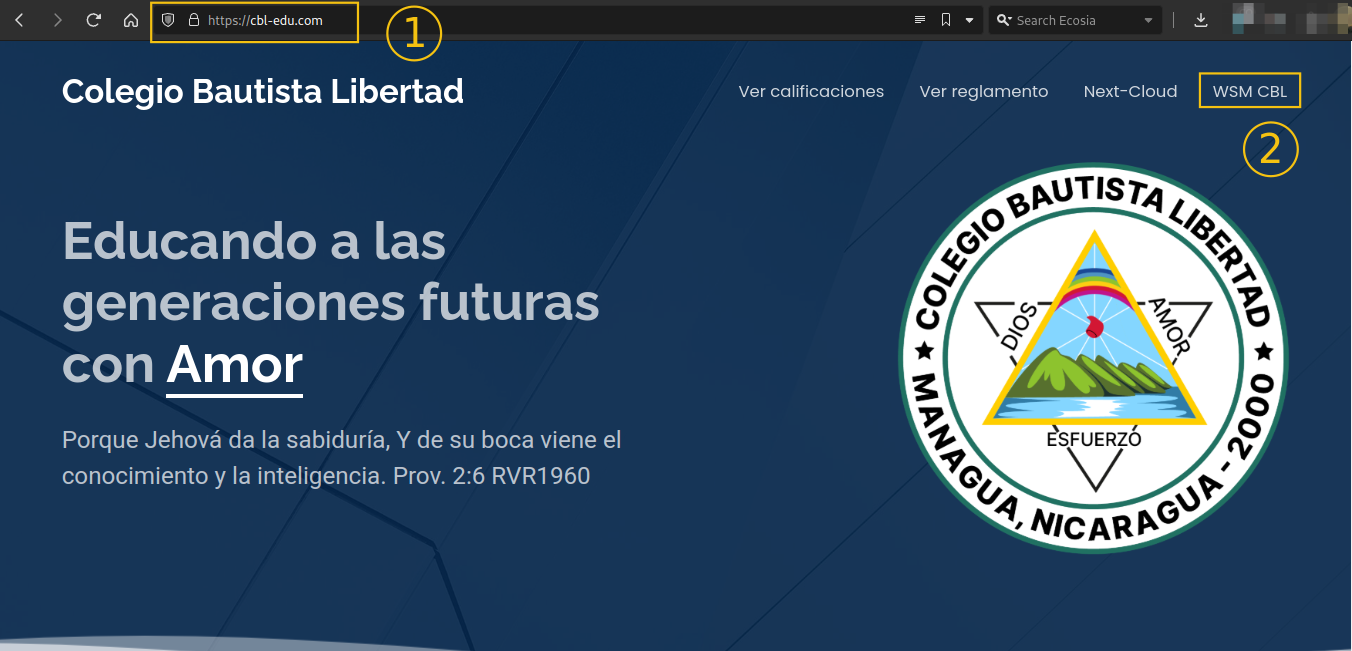
\includegraphics[width=\textwidth]{image/login.01}
        \caption{Paso 1 y 2.}
        \label{fig:login1}
    \end{figure}

    \step{3} Ingrese el correo institucional de CBL y su contraseña. Ver figura 2.

    \step{4} Se ingresa a su perfil en \wsm. Ver figura 3.

    Es preciso indicar que todo lo realizado en \wsm es parte de la información interna del colegio.
    Esto no será visible al público por medio del sitio web.
    Por tanto, es de suma importancia \textbf{no compartir sus credenciales} con ninguna persona para asegurar la integridad de los datos de la institución.
    Si perde sus credenciales recurra a dirección o bien al correo \href{mailto:soporte@cbl-edu.com}{soporte@cbl-edu.com}
    para ayudarle con su caso.

    \begin{figure}[H]
        \centering
        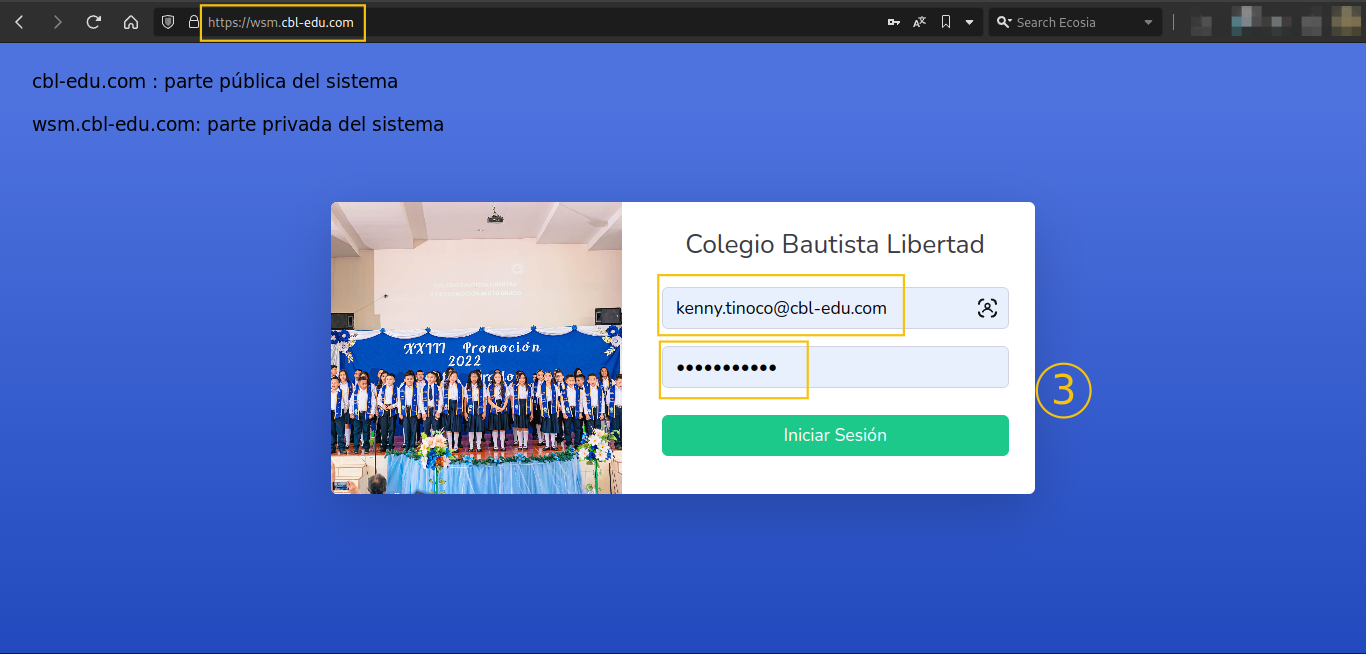
\includegraphics[width=\textwidth]{image/login.02}
        \caption{Paso 3.}
        \label{fig:login2}
    \end{figure}

    \begin{figure}[H]
        \centering
        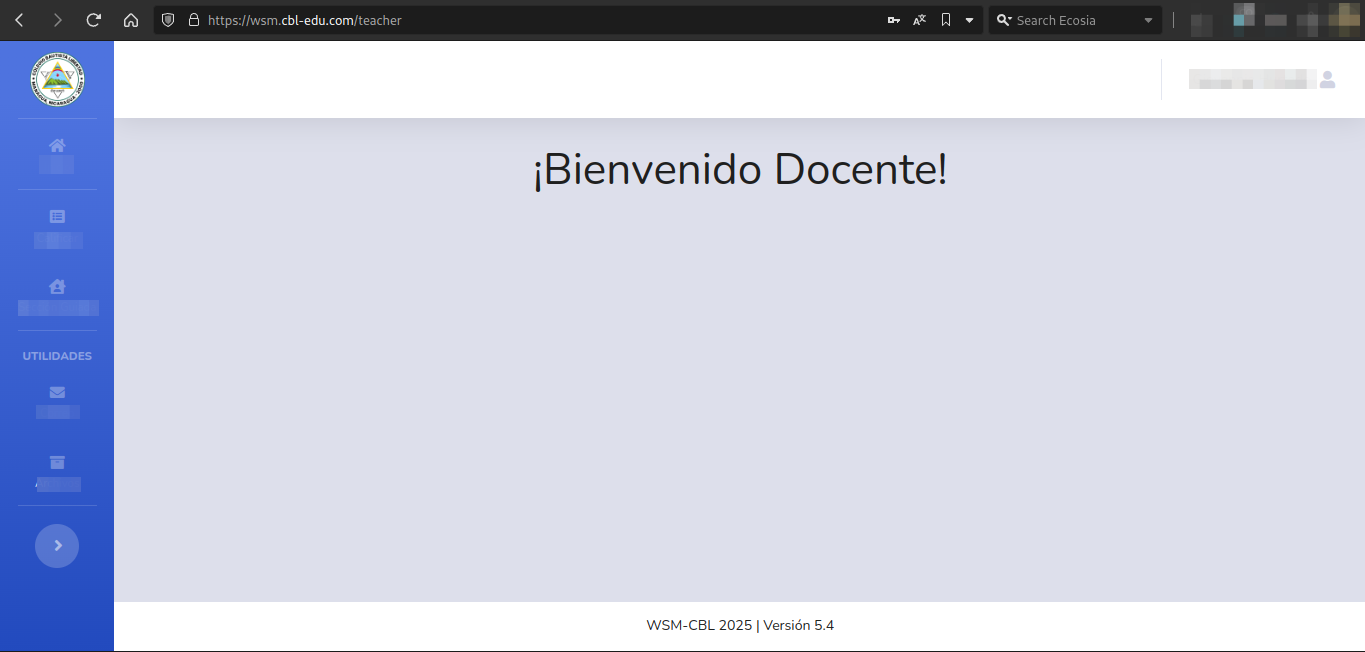
\includegraphics[width=\textwidth]{image/login.03}
        \caption{Paso 4.}
        \label{fig:login3}
    \end{figure}


    \subsection{Ver sección guiada}

    Para este caso de uso el docente debe tener una sección guida.
    Si no tiene asignada una sección esta opción se muestra vacía.

    \textbf{\large Pasos}\par

    \step{1} Iniciar sesión en el sistema.
    \step{2} Diríjase a la barra lateral izquierda y seleccione la opción ``Sección Guidada''.

    \begin{figure}[H]
        \centering
        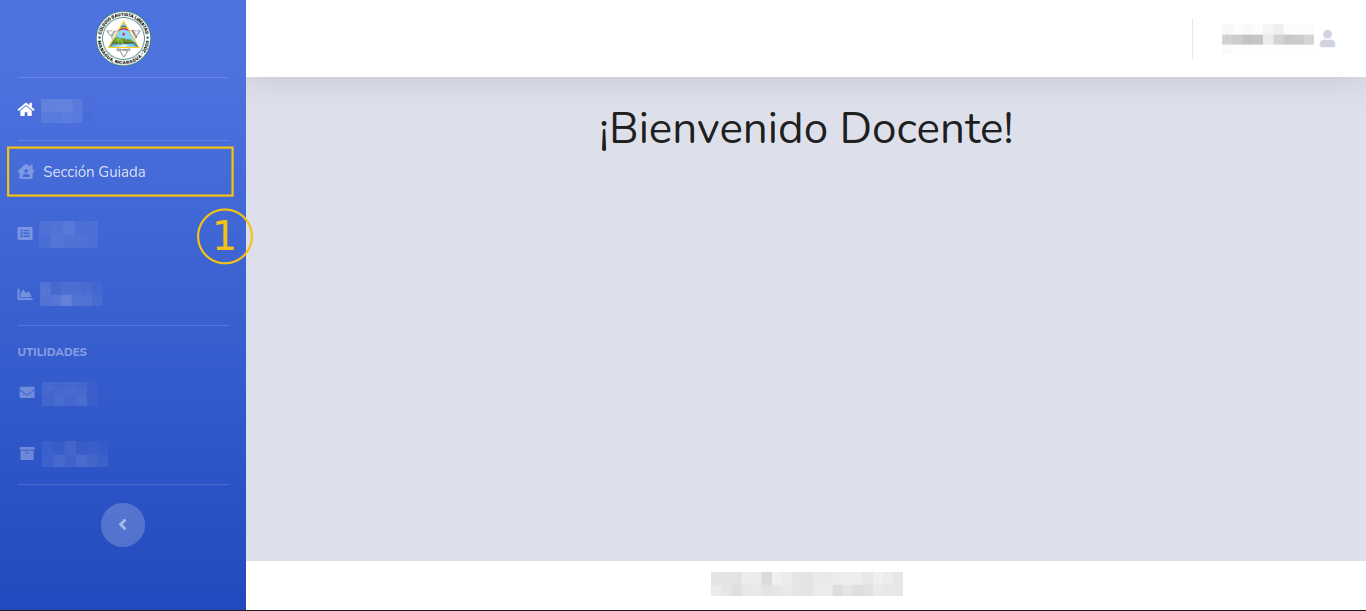
\includegraphics[width=\textwidth]{image/view.enrollment.guide.01}
        \caption{Paso 1.}
    \end{figure}

    \step{3} Se muestra la información de la sección guíada.
    \begin{itemize}
        \item Cantidad de estudiantes, capacidad de la sección y la distribución entre varones y mujeres.
        \item Lista oficial de estudiantes.
        \item Lista de asignaturas y su docente responsable.
    \end{itemize}



    \subsection{Ver información del estudiante}

    Como responsable una sección un docente necesita el acceso a la información de cada estudiante.
    El sistema \wsm registra los datos más importantes en el proceso de matrícula y el docente puede acceder a ella.

    \stepTitle

    \step{1} Ingresar a la ventana de sección guiada.
    \step{2} Elija un estudiante y selecciones los tres puntos en la parte derecha.
    \step{3} Seleccione la opción \quations{Ver perfil}.


    \subsection{Actualizar información de estudiantes}

    Al inicio de cada año lectivo se revisa y ajusta la información de cada estudiante para garantizar la integridad de los datos.
    El sistema \wsm permite que los docentes puedan actualizar la información de cada estudiante en su sección guiada.

    \stepTitle
    \step{1} Ingresar a la ventana de sección guiada.
    \step{2} Ingrese al perfil de un estudiante.
    \step{3} Actualize los datos.
    \step{4} Seleccione actualizar.

    \textbf{Nota:} La opción de actualizar la información de estudiantes no está habilitada por defecto.
    Es necesario que dirección autorice y conceda el permiso a los usuarios.


    \subsection{Registrar calificaciones}

    Para registrar calificaciones se necesita que el parcial en curso tenga su \textbf{registro de calificaciones} activo,
    En caso contrario ninguna calificación se registra.
    Sin embargo, visualizar las calificaciones ya registradas sí es posible sin necesidad del registro de calificaciones activo.

    \stepTitle
    \step{1} Iniciar sesión en el sistema.
    \step{2} Diríjase a la barra lateral izquierda y seleccione la opción \quations{Calificar}.
    \step{3} Se muestra la lista de secciones del docente.
    \step{4} Elija una sección y seleccione \quations{Ver}.
    \step{5} Se muestra la información de la sección
    \begin{itemize}
        \item Lista de estudiantes ordenados por sexo y nombre.
        \item Lista de asignaturas del docente.
        \item Campos para ingresar las calificaciones.
    \end{itemize}

    \step{6} Ingrese las calificaciones de los estudiantes en cada asignatura.
    \step{7} Ingrese las calificaciones de conducta.
    \step{8} Seleccione guardar.

    \textbf{Importante:} Si el docente imparte más de una asignatura en la misma sección, la calificación de conducta ingresada
    será la conducta para cada asignatura por separado.

    Por ejemplo, si tiene dos asignaturas en la sección y para el estudiante \quations{Jordan Tinoco} la calificación
    de conducta en la tabla es de 89, \wsm internamente registra la conducta de las dos asignaturas como 89.
    Análogamente, sucederá con una cantidad $n$ asignaturas.

    Por otra parte, el docente puede realizar correcciones a las calificaciones ingresadas mientras el registro de
    calificaciones esté activo.
    Si no ingresa las calificaciones de uno o más estudiantes, \wsm establece a cero como calificación por defecto.
    Esto nos da la facilidad de no ingresar todas las calificaciones desde el inicio y realizarlo de manera paulatina.

    \subsection{Ver historia (registro)}

    Como docente guía se necesita conocer el desempeño de los estudiantes en sus distintas asignaturas.
    El sistema \wsm permite obtener estos datos de manera sintetizada.
    Esto con el fin de reducir el trabajo que el docente de realizar en cada corte evaluativo.

    \stepTitle
    \step{1} Iniciar sesión en el sistema.
    \step{2} Diríjase a la barra lateral izquierda y seleccione la opción \quations{Registro}.
    \step{3} Se muestra tres pestañas
    \begin{itemize}
        \item Top: Muestra el promedio de los cuatro parciales para cada estudiante.
        \item Sabana: Muestra el detallado de calificaciones para cada estudiante en el parcial actual.
        \item Estadística: Muestra estadísticas de las calificaciones por parcial.
    \end{itemize}

    Estos datos pueden ser solicitados por parcial en cualquier momento, con lo cual es posible realizar un análisis
    de desempeño de los estudiantes.


    \newpage
    \section{Conclusión}

    Debido a la forma de operar del Colegio Bautista Libertad este sistema trata de ser lo menos invasivo con respecto
    a los docentes, con lo cual esta herramienta solo necesita dos aspectos del cuerpo docente; que provea de manera
    íntegra los datos de calificaciones para cada uno de sus estudiantes, y que
    vele por la correcta información de los estudiantes en el sistema.

    Teniendo presente que el éxito que \wsm pueda tener, recaerá en el uso correcto y constante de la información que se
    registre, espera digitalizar y optimizar los procesos internos del Colegio Bautista Libertad con éxito.

\end{document}